\section{Date: 2026-10-24}
\noindent \textbf{Series ID: CUURX200SS47014} 

\noindent This series is titled Consumer Price Index for All Urban Consumers: Gasoline, Unleaded Regular in Midwest - Size Class B/C and has a frequency of Monthly. The units are Index Dec 1997=100 and the seasonal adjustment is Not Seasonally Adjusted.The observation start date is 1997-12-01 and the observation end date is 2026-09-01.The popularity of this series is 1. \\ 

\noindent \textbf{Series ID: PIEATI02JPQ661N} 

\noindent This series is titled Producer Prices Index: Economic Activities: Industrial Activities: Domestic for Japan and has a frequency of Quarterly. The units are Index 2015=100 and the seasonal adjustment is Not Seasonally Adjusted.The observation start date is 1995-01-01 and the observation end date is 2022-10-01.The popularity of this series is 1. \\ 

\subsection{Raw Regression}
\noindent Regresses the two series against each other directly. A significant result here can come just as easily from both series sharing a long-run trend as from any real relationship.

\begin{center}
\begin{tabular}{lclc}
\toprule
\textbf{Dep. Variable:}               & value\_fred\_PIEATI02JPQ661N & \textbf{  R-squared:         } &     0.131   \\
\textbf{Model:}                       &             OLS              & \textbf{  Adj. R-squared:    } &     0.122   \\
\textbf{Method:}                      &        Least Squares         & \textbf{  F-statistic:       } &     14.73   \\
\textbf{Date:}                        &       Sat, 24 Oct 2026       & \textbf{  Prob (F-statistic):} &  0.000220   \\
\textbf{Time:}                        &           14:58:05           & \textbf{  Log-Likelihood:    } &   -267.69   \\
\textbf{No. Observations:}            &               100            & \textbf{  AIC:               } &     539.4   \\
\textbf{Df Residuals:}                &                98            & \textbf{  BIC:               } &     544.6   \\
\textbf{Df Model:}                    &                 1            & \textbf{                     } &             \\
\textbf{Covariance Type:}             &          nonrobust           & \textbf{                     } &             \\
\bottomrule
\end{tabular}
\begin{tabular}{lcccccc}
                                      & \textbf{coef} & \textbf{std err} & \textbf{t} & \textbf{P$> |$t$|$} & \textbf{[0.025} & \textbf{0.975]}  \\
\midrule
\textbf{const}                        &      96.1597  &        1.060     &    90.736  &         0.000        &       94.057    &       98.263     \\
\textbf{value\_fred\_CUURX200SS47014} &       0.0172  &        0.004     &     3.838  &         0.000        &        0.008    &        0.026     \\
\bottomrule
\end{tabular}
\begin{tabular}{lclc}
\textbf{Omnibus:}       & 39.712 & \textbf{  Durbin-Watson:     } &    0.070  \\
\textbf{Prob(Omnibus):} &  0.000 & \textbf{  Jarque-Bera (JB):  } &   82.712  \\
\textbf{Skew:}          &  1.575 & \textbf{  Prob(JB):          } & 1.09e-18  \\
\textbf{Kurtosis:}      &  6.150 & \textbf{  Cond. No.          } &     704.  \\
\bottomrule
\end{tabular}
%\caption{OLS Regression Results}
\end{center}

Notes: \newline
 [1] Standard Errors assume that the covariance matrix of the errors is correctly specified.

\begin{figure}
\centering
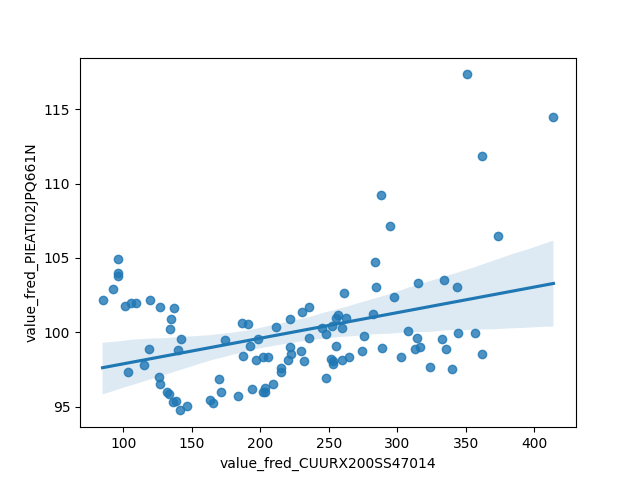
\includegraphics[scale = 0.9]{plots/plot_2026-10-24.png}
\caption{Raw Regression Plot for 2026-10-24}
\end{figure}
\newpage
\subsection{Detrended Regression}
\noindent Regresses the residuals of each series after removing its own linear time trend, so a shared trend can no longer drive the result on its own. A relationship that stays significant here is better evidence of a genuine link between the two series.

\begin{center}
\begin{tabular}{lclc}
\toprule
\textbf{Dep. Variable:}                          & value\_fred\_PIEATI02JPQ661N\_detrended & \textbf{  R-squared:         } &     0.050   \\
\textbf{Model:}                                  &                   OLS                   & \textbf{  Adj. R-squared:    } &     0.041   \\
\textbf{Method:}                                 &              Least Squares              & \textbf{  F-statistic:       } &     5.206   \\
\textbf{Date:}                                   &             Sat, 24 Oct 2026            & \textbf{  Prob (F-statistic):} &   0.0247    \\
\textbf{Time:}                                   &                 14:58:05                & \textbf{  Log-Likelihood:    } &   -267.05   \\
\textbf{No. Observations:}                       &                     100                 & \textbf{  AIC:               } &     538.1   \\
\textbf{Df Residuals:}                           &                      98                 & \textbf{  BIC:               } &     543.3   \\
\textbf{Df Model:}                               &                       1                 & \textbf{                     } &             \\
\textbf{Covariance Type:}                        &                nonrobust                & \textbf{                     } &             \\
\bottomrule
\end{tabular}
\begin{tabular}{lcccccc}
                                                 & \textbf{coef} & \textbf{std err} & \textbf{t} & \textbf{P$> |$t$|$} & \textbf{[0.025} & \textbf{0.975]}  \\
\midrule
\textbf{const}                                   &   -3.933e-12  &        0.353     & -1.11e-11  &         1.000        &       -0.701    &        0.701     \\
\textbf{value\_fred\_CUURX200SS47014\_detrended} &       0.0131  &        0.006     &     2.282  &         0.025        &        0.002    &        0.025     \\
\bottomrule
\end{tabular}
\begin{tabular}{lclc}
\textbf{Omnibus:}       & 38.979 & \textbf{  Durbin-Watson:     } &    0.075  \\
\textbf{Prob(Omnibus):} &  0.000 & \textbf{  Jarque-Bera (JB):  } &   77.149  \\
\textbf{Skew:}          &  1.582 & \textbf{  Prob(JB):          } & 1.77e-17  \\
\textbf{Kurtosis:}      &  5.916 & \textbf{  Cond. No.          } &     61.4  \\
\bottomrule
\end{tabular}
%\caption{OLS Regression Results}
\end{center}

Notes: \newline
 [1] Standard Errors assume that the covariance matrix of the errors is correctly specified.

\begin{figure}
\centering
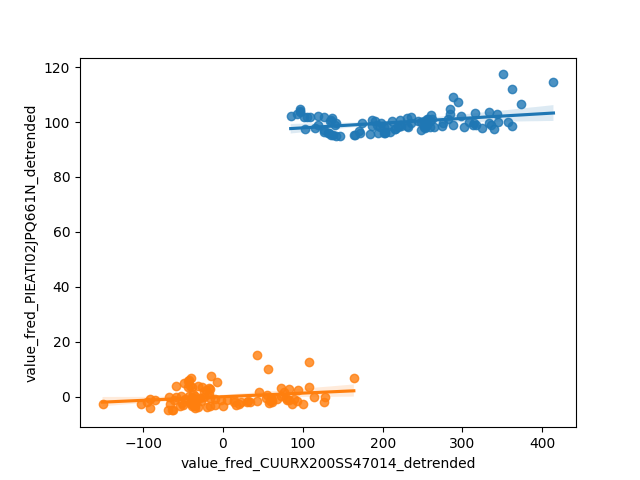
\includegraphics[scale = 0.9]{plots/plot_2026-10-24_detrended.png}
\caption{Detrended Regression Plot for 2026-10-24}
\end{figure}
\newpage
